\documentclass[12pt, letterpaper]{article}
\usepackage[utf8]{inputenc}
\usepackage[margin=2cm]{geometry}
\usepackage{amsmath}
\usepackage{amssymb}
\usepackage{graphicx}
\usepackage{cancel}
\usepackage{fancyhdr}
\usepackage{float}

\graphicspath{ {./bilder/} }

\title{ \begin{huge}
\textbf{Portfolio Assignment 2}
\end{huge} }

\author{Candidate 25}
\date{}

\rfoot{\thepage}
\newcommand{\bs}{\boldsymbol}
\newcommand{\mbf}{\mathbf}

\begin{document}
\maketitle
  \section*{Problem 1}
    \subsection*{(1a)}
      \begin{figure}[H]
        \caption{Decision boudary of a logistic descrimination classifier}
        \centering
        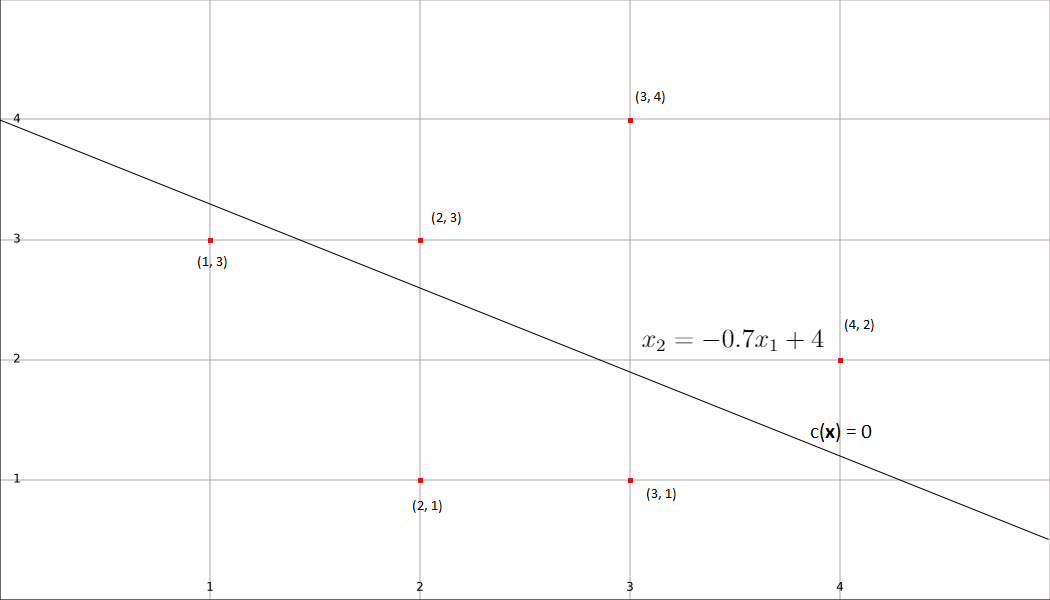
\includegraphics[width=\textwidth,keepaspectratio=true,height=\textheight-\the\textundbildtextheight]{decisionboundary_1a}
      \end{figure}\\
      In the plot above we see the points from the training set: $\{(\mbf{x}^i, y^i)\}_{i=1}^6$ as red points. $\mbf{x}^i$ is the trainig data, and $y^i$ is the ground truth. The line going somewhat diagonally across the plot is the decision boundary. This is used to classify the points above the line as $y^i = 0$, and points underneath the decision boundary as $y^i = 1$. This decision boundary is given by the equation:
      \begin{align} \label{eq1}
        C(\mbf{x}) = \bs{w}^T \cdot \mbf{x} + w_0
      \end{align}
      Which put simply, assigns a class to an vector $\mbf{x}^i$. If the vector after being put into\\ $C(\mbf{x}) > 0 \implies \mbf{x} \rightarrow C^1$ or the opposite case where $C(\mbf{x}) < 0 \implies \mbf{x} \rightarrow C^2$. Which means at $C(\mbf{x}) = 0$ we are on the decision boundary. From this we can derive the equation of the decision boundary, $x_2 = -\frac{w_1}{w_2}\cdot x_1 - \frac{w_0}{w_2}$. In my guess for the decision boundary i used $w_1 = -0.7, w_2 = 1$ and $ w_0 = 4$ to give the decision boundary of $x_2 = -0.7 \cdot x_1 + 4$. Here we see that the weights, $\bs{w}$ of the classifier determines the slope of the decision boundary, whereas the bias, $w_0$ determines the intercept with the second axis, $x_2$.\\
      \newline
      To figure out the distance between the origin, $\bs{O}$, and the decision boundary we can calulate this with the formula,
      \begin{align*}
        d = \frac{w_0}{\|\bs{w}\|} = \frac{4}{\sqrt{(-0.7)^2 + 1^2}} \approx \underline{\underline{3,277}}
      \end{align*}\\
      Now i shall demonstrate how this decision boundary could give us a decision rule, based on the estimated weights and biases. Consider a test point,
      \begin{align*}
        \mbf{x}^t =
        \begin{bmatrix}
          x_1^t \\
          x_2^t \\
        \end{bmatrix}
      \end{align*}
      this point will from what I stated earlier follow the  decision rule,
      \[
        \begin{cases}
          C(\mbf{x^t}) > 0, & y^t = 0\\
          C(\mbf{x^t}) \leq 0, & y^t = 1\\
        \end{cases}
      \]
      Here i have also made the assumption that if  $C(\mbf{x^t}) = 0$ then $\mbf{x^t}$ is assigned to $y^t = 1$, althoug in reality this is quite rare.

    \subsection*{(1b)}
      % \begin{figure}[h]
      %   \caption{Confusion matrix and accuracy of test on trained model.}
      %   \centering
      %   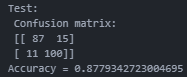
\includegraphics[width=5cm]{confmat1b}
      % \end{figure}
      After having trained my logistic discrimination model on the \textit{seals\_train.csv} file, and the used the trained weights to classify the test data. I produce with the \textit{seals\_test.csv} file the confusion matrix:\\
      \[
        \text{confusion matrix} =
        \begin{bmatrix}
          87 & 15  & \\
          11 & 100 & \\
        \end{bmatrix}
        \text{, and accuracy} \approx \underline{0.878}
      \]
      Which means the model classified 87 class 0's correctly, 11 class 1's as class 0's, 15 class 0's as class 1's and 100 class 1's correctly.
    \newpage
    \subsection*{(1c)}
      \begin{figure}[H]
        \caption{The Reciever Operating Characteristic}
        \centering
        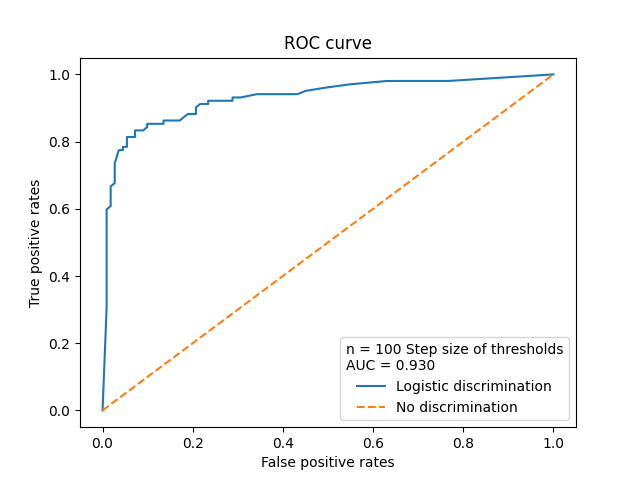
\includegraphics[width=14cm]{ROC}
      \end{figure}\\
      The ROC curve represents\\

      \noindent For the Area Under the Curve score i got AUC $ \approx \underline{0.930}$ by using \textit{sklearn.metrics} built-in function for calculating the AUC score.
    \subsection*{(1d)}
      For this task I have created a function which classifies seal images corresponding to a given index, called \textit{show\_image}. Furthermore I use this function to show 5 random images which I know my classifier correctly classified in task (1b), and 5 random images I know are incorrectly classified.
      \begin{figure}[H]
        \caption{Pictures of correctly classified seals}
        \centering
        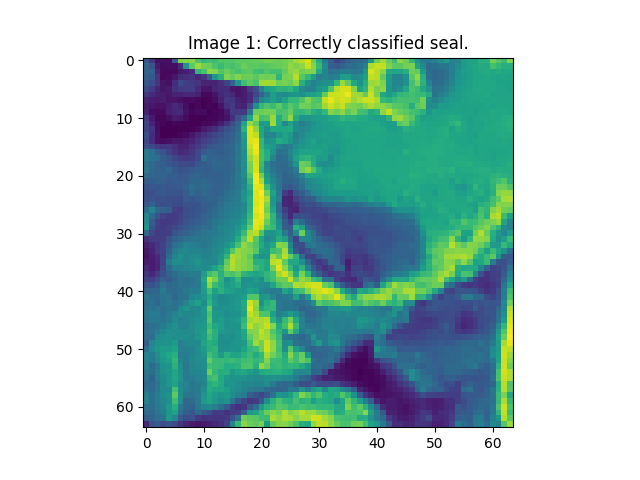
\includegraphics[width=8cm]{corr1}
        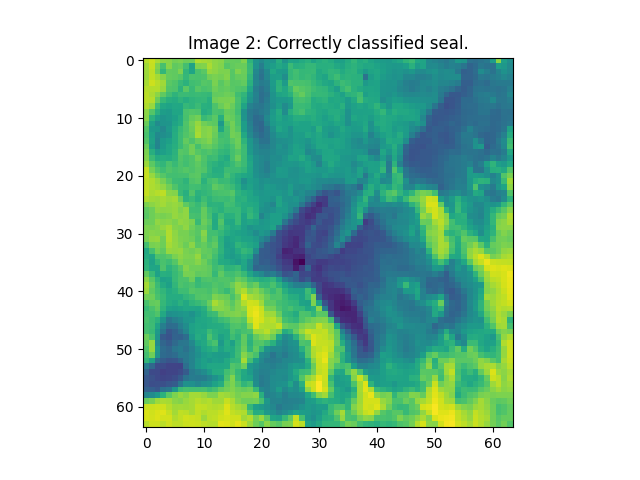
\includegraphics[width=8cm]{corr2}
        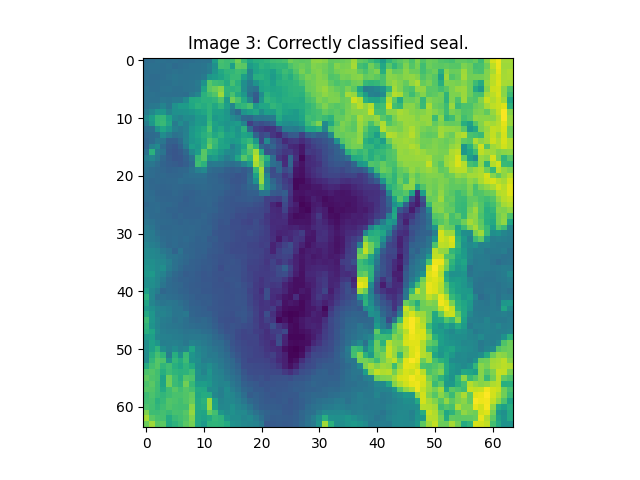
\includegraphics[width=8cm]{corr3}
        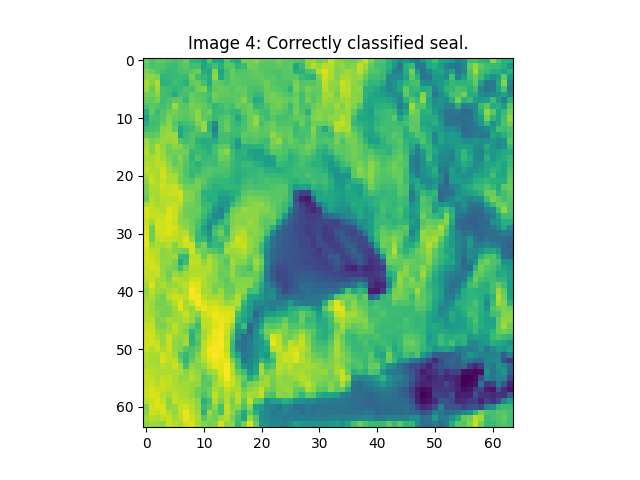
\includegraphics[width=8cm]{corr4}
        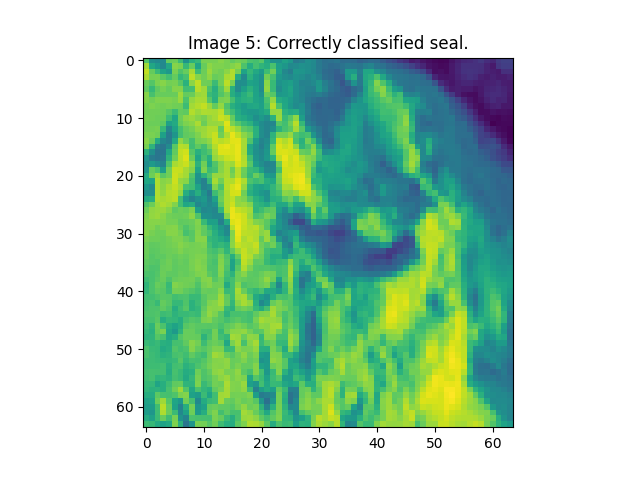
\includegraphics[width=8cm]{corr5}
      \end{figure}\\
      \begin{figure}[H]
        \caption{Pictures of not correctly classified seals}
        \centering
        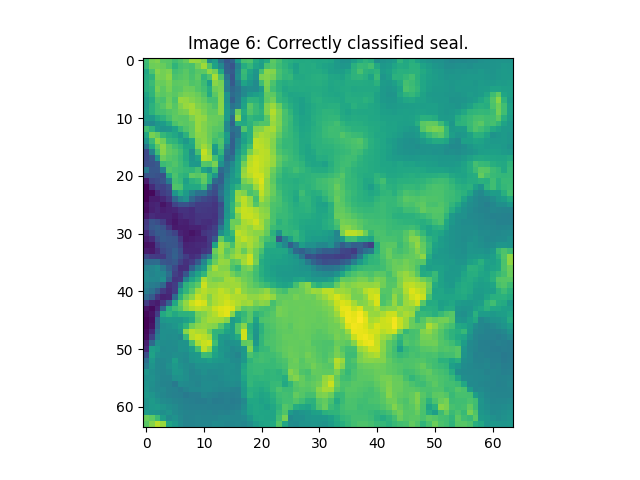
\includegraphics[width=8cm]{notcorr6}
        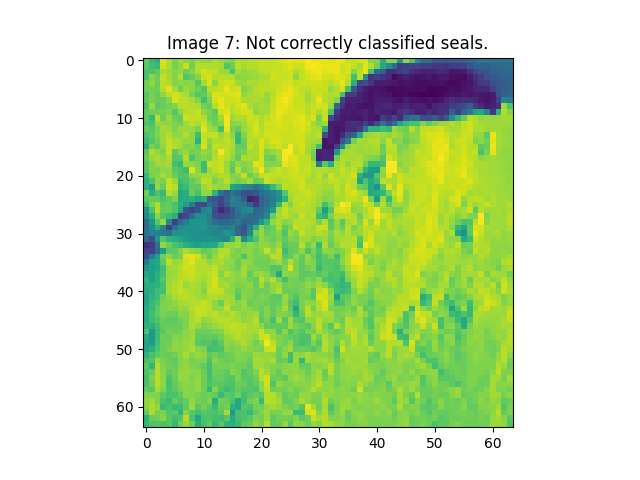
\includegraphics[width=8cm]{notcorr7}
        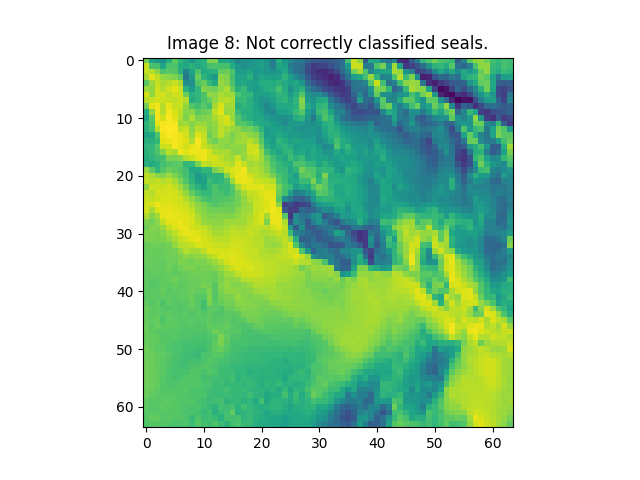
\includegraphics[width=8cm]{notcorr8}
        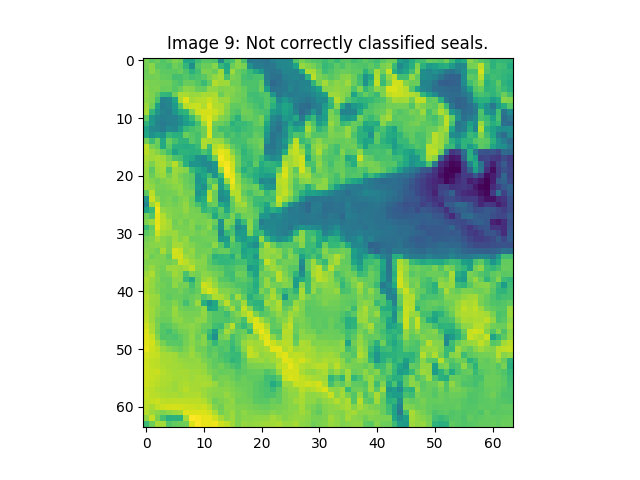
\includegraphics[width=8cm]{notcorr9}
        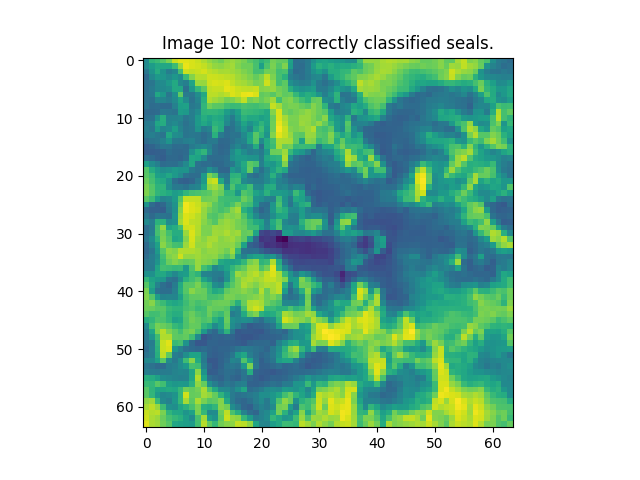
\includegraphics[width=8cm]{notcorr10}
      \end{figure}\\
      \noindent In Figure 3. the pictures are of either \textit{Harp seal pups} or \textit{Hooded seal pups}, where the algorithm has classified theese seals correctly. Whereas in Figure 4. the pictures are of either \textit{Harp seal pups} classified as \textit{Hooded seal pups}, or \textit{Hooded seal pups} classified as \textit{Harp seal pups}.\\
      \\
      This leads to a question, what are the possible reasons as to why the pictures in Figure 4. are misclassified. By studying theese example photos I belive one reason to this comes from not the whole seal being present in the image. An exmple of this we see in Image 9. The seal is located between approximately pixel 50 to pixel 64 along the first axis, and pixels 10 to 30 along the second axis. Where not the whole seal is present, althoug we tell the classifier there is a seal in the image. This leads to making a sort of edjucated guess, since not all of the features neccesary to make a correct classification is present.\\
      In image 8. it seems as though the lack of a good image resolution may be hiding a lot of the features the classifier neeeds to make a correct decision, and hence it misclassifies the seal.\\
      Image 10. demonstrates a noisy image where a lot of the features of the seal is hidden due to lots of darker areas, and very bright areas making it hard to pinpoint where the seal begins and ends.\\
      In conclusion, the reason as to why the classifier fails to make a correct decision I belive arise when the images hides the distinct features of the seal.
  \section*{Problem 2}
    \subsection*{(2a)}
      \begin{figure}[H]
        \caption{2-dimensional plot of training set $\{(\mbf{x}^i, y^i)\}_{i=1}^6$, and decision boundary of a decision tree.}
        \centering
        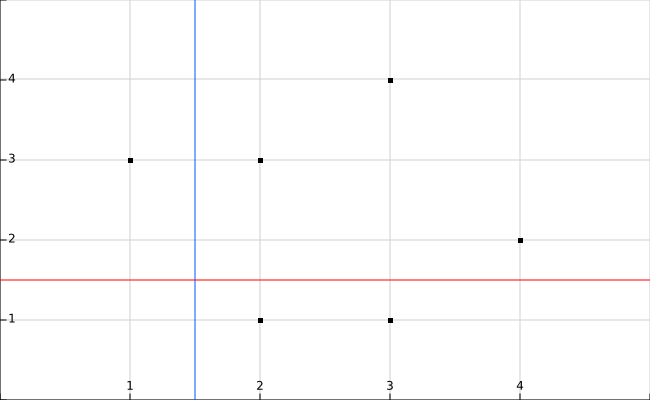
\includegraphics[scale=0.75]{decisionboundary_2a}
      \end{figure}\\
      This plot illustrates the two decision boundaries needed to classify the training set with zero errors. Here I have used two boundaries. The first going from $x_1 = 1.5$ spanning the secound axis, and the second going from $x_2 = 1.5$ spanning the first axis.\\
      \begin{figure}[H]
        \caption{Decision tree for training set.}
        \centering
        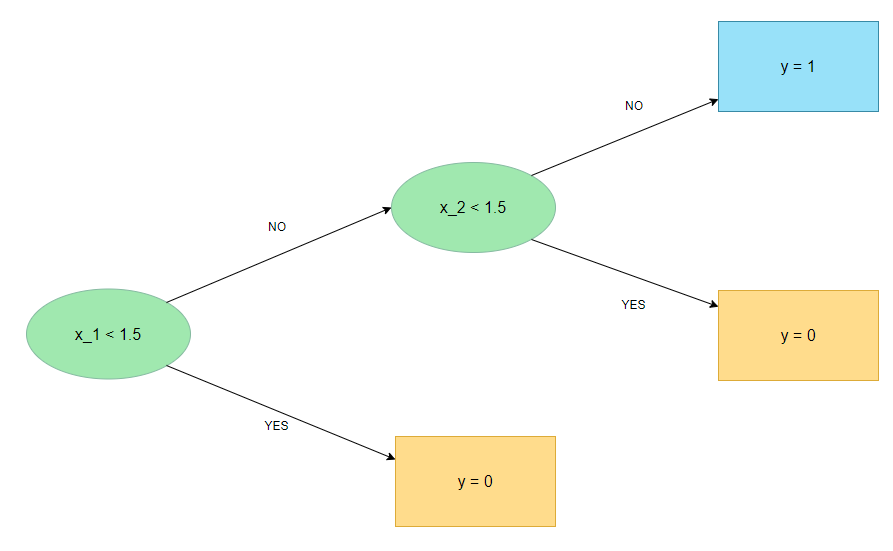
\includegraphics[scale=0.6]{DescisionTree}
      \end{figure}\\
      \noindent From this decision tree we see that we can create a IF-THEN rule which describes how the tree would classify the datapoint:
      \[
        \mbf{x}^t =
        \left[
          \begin{array}{ccc}
            x_1^t \\
            x_2^t \\
          \end{array}
        \right]
      \]
      This means that, \\
      IF: $x_1^t < 1.5$, THEN $\mbf{x}^t \rightarrow y^t = 0$\\
      IF: $x_1^t \geq$ AND $x_2^t < 1.5$ THEN $y^t = 0$\\
      IF: $x_1^t \geq$ AND $x_2^t \geq 1.5$ THEN $y^t = 1$
  \section*{Problem 3}
    \subsection*{(3a)}
      3a
\end{document}
